\documentclass{scrartcl}

\usepackage[utf8]{inputenc}
\usepackage{ngerman}
\usepackage{amsmath}
\usepackage{amssymb}
\usepackage{a4wide}
\usepackage{todonotes}
\usepackage{graphicx}

\title{GCN}

\begin{document}

\maketitle

\section{CNNs auf variierenden Größen}

Meistens werden Bilder für die Eingabe in ein CNN gecroppt oder gewarped, damit sie einer fixen Bildgröße (z.B. $244 \times 244$) entsprechen.
Dabei gehen aber Bildteile verloren oder werden geometrisch gestreckt, so dass sie nicht mehr naturgetreu sind.
Desweiteren helfen Bilder mit verschiedenen Größen dabei, skalierungsinvariant zu trainieren und reduzieren Overfitting.
Warum brauchen CNNs eine fixe Größe?
Ein CNN besteht aus zwei Teilen, Convolutional Layern und Fully-Connected Layern.
Die Convolutional Layer opeieren über einem beweglichen Fenster.
Convolutional Layer brauchen eigentlich keine fixe Größe und können Feature Maps beliebiger Größe generieren.
Das ist der Ursache geschuldet, dass wir immer nur einen Bildausschnitt betrachten und shared Weights and Biase haben.
Die Fully-Connected Layer allerdings haben diesen Vorteil nicht, sie brauchen stets eine feste Anzahl an Neuronen.
Beim Übergang zwischen Convolution und Fully-Connected kriegen wir deshalb Probleme.

Ein Layer zwischen diesen beiden Teilen mit der Aufgabe, eine beliebige Größe von Feature Maps auf eine feste Anzahl an Neuronen zu mappen, könnte dieses Problem beseitigen.
Dieser Layer wird auch SPP genannt (\emph{Spatial Pyramid Pooling}).

\subsection{SPP Layer}

\begin{figure}[h]
  \centering
  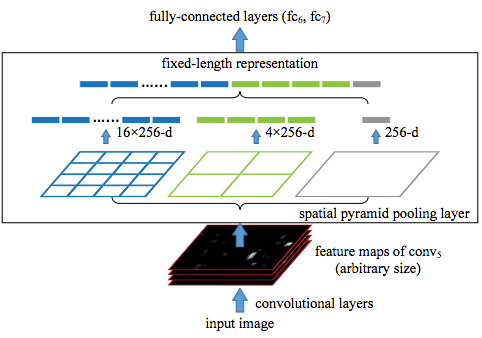
\includegraphics[width=.6\textwidth]{images/spp}
\end{figure}

Aus der letzten Convolution (z.B. $256$ Feature Maps, d.h. Shape \texttt{[-1, -1, 256]}) werden mehrere \emph{Spatial Bins} verschiedener Größen über \emph{Max-Pooling} berechnet.
In jedem Bin werden die Features Maps gepoolt mit Größe $kM$, wobei $M$ die Anzahl an Bins ist und $k$ die Anzahl an Feature Maps.

Angenommen wir haben eine Bildgröße von $224 \times 224$ und ein CNN, dass uns nach der Convolution Shapes der Form \texttt{[13, 13, 256]} liefert mit $a \times a = 13 \times 13$.
Sagen wir wir wollen $3$ 3 Bins aufbauen mit $l = 3$:
Dann berechnen sich die Pooling Windows mit $\lceil \frac{a}{n} \rceil$ und Strides mit $\lfloor \frac{a}{n} \rfloor$ mit $n = 1, 2, 3$.

Dann können wir z.B. 3 mal Max Pooling auf diesen Daten anwenden:

\begin{enumerate}
  \item $3 \times 3 \Rightarrow$ Size $5$, Stride $4$
  \item $2 \times 2 \Rightarrow$ Size $7$, Stride $6$
  \item $1 \times 1 \Rightarrow$ Size $13$ Stride $13$
\end{enumerate}

Dann ergibt dies:

\begin{equation}
  3 \times 3 \times 256 + 2 \times 2 \times 256 + 1 \times 1 \times 256 = 3584
\end{equation}

Diese Neuronen können wir nun mit unseren Fully Connected Neuronen verbinden.

Jetzt testen wir noch eine unterschiedliche Bildgröße von $180 \times 180$.
Dann hat das CNN nach der Convolution die Shape \texttt{[10, 10, 256]} mit $a \times a = 10 \times 10$.

\begin{enumerate}
  \item $3 \times 3 \Rightarrow$ Size $4$, Stride $3$
  \item $2 \times 2 \Rightarrow$ Size $5$, Stride $5$
  \item $1 \times 1 \Rightarrow$ Size $10$ Stride $10$
\end{enumerate}

Auch das ergibt:

\begin{equation}
  3 \times 3 \times 256 + 2 \times 2 \times 256 + 1 \times 1 \times 256 = 3584
\end{equation}

\section{Graph Convolutional Networks}

\begin{itemize}
  \item großes wissenschaftliches Problem, willkürliche Graphen in ein neuronales Netz zu füttern
  \item Bereich bisher dominiert von kernelbasierten Methoden, graphbasierter Regularisierung oder ähnlichem
  \item Es gibt eine Ansätze, der neuste ist ein \emph{spektraler}
  \item spektraler Ansatz gilt als langsam
  \item das ganze zählt zu dem Bereich des \emph{Semi-unsupervised Learning}, das bedeutet, dass wir einen Teil des Graphen gelabelt haben und basierend auf seiner Graphstruktur, den Rest labeln wollen.
\end{itemize}

\subsection{Definitionen}

\begin{itemize}
  \item Wir wollen eine Funktion von Merkmalen auf einem Graphen $\mathcal{G} = (\mathcal{V}, \mathcal{E})$ lernen
  \item \textbf{Eingaben:}
  \begin{itemize}
    \item Eine Merkmalsbeschreibung $x_i$ für jeden Knoten $i$ dargestellt als eine Merkmalsmatrix $X = N \times D$, wobei $N$ Anzahl der Knoten und $D$ Anzahl der Merkmale
    \item Eine repräsentative Beschreibung einer Graphstruktur in Matrixform, normalerweise eine Adjazenzmatrix $A$
  \end{itemize}
  \item \textbf{Ausgabe}:
  \begin{itemize}
    \item eine Merkmalsbeschreibung $Z = N \times F$ für jeden Knoten, wobei $F$ Anzahl der Ausgabefeatures für \underline{einen} Knoten
  \end{itemize}
\end{itemize}

Jede Schicht des neuronalen Netzes kann über eine nicht-lineare Funktion

\begin{equation}
  H^{(l+1)} = f(H^{(l)}, A)
\end{equation}

beschrieben werden, wobei $H^{(0)} = X$ und $H^{(L)} = Z$ mit $L$ Anzahl der Schichten.

Die Propagationsregel ist dann zum Beispiel:

\begin{equation}
  f(H^{(l)}, A) = \sigma(AH^{(l)}W^{(l)})
\end{equation}

wobei, $\sigma$ eine nicht lineare Aktivierungsfunktion ist (z.B. \texttt{ReLU}) und $W^{(l)}$ eine Gewichtsmatrix für den $l$ten Layer.

Sagen wir $A$ ist eine $n \times n$ Matrix, die über mehrere Graphen hinweg variabel ist.
Graph $1$ hat zum Beispiel $n = 100$ Knoten, wohingegen Graph $2$ nur $n = 80$.
$H^{(l)}$ ist eine $n \times f_j$.
Die Anzahl an Features pro Layer sind unabhängig vom Graphen und immer gleich.
Dann ist $AH^{(l)}$ eine $n \times f_j$ Matrix.
$W^{(l)}$ ist eine $f_{j} \times f^{j+1}$ Matrix.
Damit ist die Gewichtsmatrix unabhängig der Knotenanzahl und kann auch für verschiedene große Graphen genutzt werden.
Die Gleichheit von $W^{(l)}$ liefert uns den Convolution Gedanken (Shared Weights).
Dann ist $H^{(l+1)}$ eine $n \times f_{j+1}$ Matrix.

Am Ende der Convolution hin zum Fully-Connected muss dann $n \times f_{j}$ gepoolt werden, damit es immer gleich viele Eingabeneuronen gibt (siehe SPP).

$A$ muss jedoch leicht modifziert werden, denn eine Multiplikation mit $A$ summiert alle Feature Vectors der lokalen Nachbarschaftsknoten auf, jedoch ohne den betrachteten Knoten (falls Knoten keine Kante zu sich selbst).
Wir können das fixen, in dem wir für jeden Knoten eine Kante sich zu selbst hinzufügen in dem wir $A$ mit der Identitätsmatrix addieren.

Desweiteren ist $A$ nicht normalisiert, das bedeutet, dass eine Multiplikation mit $A$ die Featurevectors komplett anders skaliert.
$A$ kann zum Beispiel normalisiert werden, in dem alle Reihen zu Eins aufsummiert werden.

\begin{equation}
  D_{ii} = \sum_j A_{ij}
\end{equation}

beziehungsweise

\begin{equation}
  D^{-1}_{ii} = \frac{1}{\sum_j A_{ij}}
\end{equation}

Matrixnormalisierung dann zum Beispiel $D^{-1}A$ oder $D^{-\frac{1}{2}}AD^{-\frac{1}{2}}$.

Der erste Layer würde dann die Features eines Knotens mit denen der direkten Nachbarschaft kombinieren.
Ein weiterer Layer würde, diess für alle Wege mit Länge $2$ tun und so weiter.

Dies entspricht in etwa einer generaliserten Version des Weisfeiler-Lehman Algorithmus auf Graphen:

Für alle Knoten $v_i \in \mathcal{G}$:
\begin{enumerate}
  \item Sammle Merkmale $\lbrace h_{v_j} \rbrace$ für alle Nachbarschaftsknoten ${ v_j }$
  \item Update Knotenmerkmal $h_{v_i} \leftarrow \text{hash}(\sum_j h_{v_j})$
Wiederhole $k$-mal oder bis Konvergenz.
\end{enumerate}

Jedem Knoten wird also ein Merkmal zugeordnet, dass seine Rolle im Graphen beschreibt.
Dies funktioniert jedoch nicht gut für z.B. reguläre Graphen, bei dem jeder Knoten gleich viele Kanten besitzt.
Der Weisfeiler-Lehman Algorithmus wird oft benutzt, um Graphisomorphismen zu bestimmen.

\subsection{Klassifierung eines Graphen}

Wie kann dieses Model genutzt werden, um einen Graphen zu klassifizieren?
Wir erhalten $N \times F$ Features für einen Graphen nach $x$ vielen Convolutions.
$F$ kann natürlich dann auch die Anzahl der Klassen sein.

Weiteres Vorgehen:
Wir wollen nicht einzelne Knoten labeln, sondern das gesamte Bild bzw.\ den gesamten Graphen.
Diese Features beschreiben den Knoten sowie seine direkte und indirekte Nachbarschaft.
Die Knoten müssten jetzt eigentlich noch geeignet gelabelt werden und können dann in ein Netz gefüttert werden.

Wir können Spatial Informationen ausnutzen, wir wissen wie der Graph in der Lage aussieht.
Das sollte man sich ruhig zu nutze machen.

\subsection{Offene Fragen}

Adjazenzmatrix mit Gewichten? Wie ist das mit der Identität? Gewichte müssten ja eigentlich umgekehrt werden damit nahe Knoten (niedriges Gewicht) mehr Einfluss haben.

\section{Graph Pooling / Graph Clustering}


\section{Graph Labeling}

Jeder Ansatz von Graph hat zur Folge, dass wir irgendeine \emph{eindeutige} Sortierung von Knoten auf dem Graphen brauchen.
Wenn wir das nicht haben, dann haben zwei absolut gleiche Graphen mit unterschiedlicher Sortierung einen unterschiedlichen Output im Netz.
Das geht natürlich nicht.

Deswegen gibt es den \emph{Isomorphismus} und \emph{Automorphismus}.

\end{document}
